\chapter{Testing}

\section{Test strutturale}

\subsection{\texttt{creaOrdine()}}

\paragraph{Codice Java}

\inputminted[breaklines,tabsize=4,obeytabs]{java}{chapters/testing_white_box/creaOrdine.java}

\vfill

\pagebreak

\paragraph{Control Flow Graph} \mbox{}\newline

\noindent\begin{minipage}[t]{0.65\linewidth}
	\vspace{0pt}
	Il numero di cammini linearmente indipendenti è detto \emph{numero ciclomatico} di McCabe, e può essere calcolato equivalentemente in uno dei modi seguenti. Sia $G$ il grafo della funzione, allora risulta:
	\begin{enumerate}
		\item $V(G) = E - N + 2$ in cui $E = \text{\#archi in } G$, $N = \text{\#nodi in } G$
		\item $V(G) = P + 1$ con $P = \text{\#predicati in } G$
		\item $V(G) = R + 1$ con $R = \text{\#regioni chiuse in } G$
	\end{enumerate}%
	Nel nostro caso:%
	\begin{itemize}
		\item $E = 15$
		\item $N = 12$
		\item $P = 4$
		\item $R = 4$
	\end{itemize}%
	\begin{enumerate}
		\item $V(G) = E - N + 2 = 15 - 12 + 2 = 5$
		\item $P + 1 = 5$
		\item $R + 1 = 5$
	\end{enumerate}%
	\noindent I cammini di base sono:
	\begin{enumerate}
		\item 0-1
		\item 0-2-3-8-10
		\item 0-2-3-8-9-10
		\item 0-2-3-4-5-7-3-8-10
		\item 0-2-3-4-5-6-7-3-8-10
	\end{enumerate}
\end{minipage}
\hfill
\noindent
\begin{minipage}[t]{0.34\linewidth}
	\vspace{0pt}
	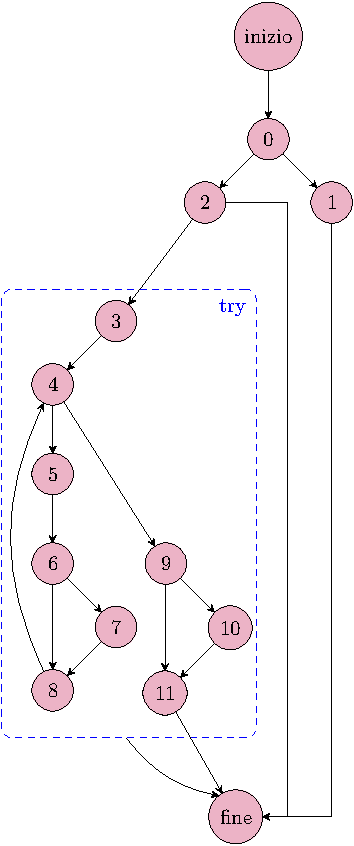
\includegraphics{chapters/testing_white_box/cfg_creaOrdine.pdf}
\end{minipage}

\vfill
\pagebreak

\paragraph{Test suite strutturale}
